\documentclass[11pt]{article}

\usepackage{hyperref}
\usepackage{tikz}
\usetikzlibrary{snakes}

\title {{Functional requirements}}
\author {Lucie-Aim\'{e}e Kaffee}
\date{}

\begin {document}

\section{Deployment cycles}
Since there were different steps of deployments, it was necessary to split up the functional requirements and built up the requirements in every step on the ones before. \\
The ideal timeline would look like this
\\ 
\\
  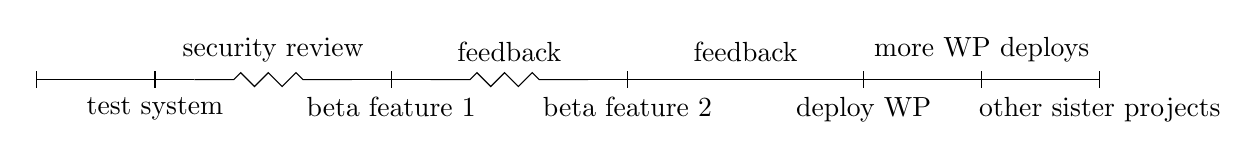
\begin{tikzpicture}[snake=zigzag, line before snake = 5mm, line after snake = 5mm]
    % draw horizontal line   
    \draw (0,0) -- (2,0);
    \draw[snake] (2,0) -- (4,0);
    \draw (4,0) -- (5,0);
    \draw[snake] (5,0) -- (7,0);
    \draw (7,0) -- (13.5,0);

    % draw vertical lines
    \foreach \x in {0,1.5,4.5,7.5,10.5,12,13.5}
      \draw (\x cm,3pt) -- (\x cm,-3pt);

    % draw nodes
    \draw (0,0) node[below=3pt] {} node[above=3pt] {$   $};
    \draw (1.5,0) node[below=3pt] {test system} node[above=3pt] {};
    \draw (3,0) node[below=3pt] {} node[above=3pt] {security review};
    \draw (4.5,0) node[below=3pt] {beta feature 1} node[above=3pt] {};
    \draw (6,0) node[below=3pt] {} node[above=3pt] {feedback};
    \draw (7.5,0) node[below=3pt] {beta feature 2} node[above=3pt] {};
    \draw (9,0) node[below=3pt] {} node[above=3pt] {feedback};
    \draw (10.5,0) node[below=3pt] {deploy WP} node[above=3pt] {};
    \draw (12,0) node[below=3pt] {} node[above=3pt] {more WP deploys};
    \draw (13.5,0) node[below=3pt] {other sister projects} node[above=3pt] {};
  \end{tikzpicture}

\subsection{wmflabs}
To have a possibility to present the extension from the beginning, there was a test setup, available on \href{articleplaceholder.wmflabs.org/mediawiki}{wmflabs}. That test setup was specifically made to get a first idea of what the aims of the project are and was not intended to be used. 

\subsection{beta feature}
The next step was to deploy the extension as a beta feature. While having certain requirements for the test set up, the beta feature was supposed to be actually used by the community and therefore needed to fulfil more requirements, building up on what was already archived in the step before. 

\subsection{deploy to a Wikipedia}
Finally the extension would be deployed to the first wiki and therefore again needed to match other requirements again. 


 

\end {document}